\documentclass{beamer}
\usepackage[utf8]{inputenc}
\usepackage[english]{babel}

% -- Including some standard packages --
\usepackage{graphicx}
\usepackage{soul}
\usepackage{hyperref}
\usepackage{colortbl}
\usepackage{dsfont}
\usepackage{soul}

% -- Choosing theme --

\usetheme{Boadilla}
\usecolortheme{whale}
\setbeamercolor{alerted text}{fg=purple} % Making alerted text non-red

% Tikz
\usepackage{tikz,tikz-3dplot,tikz-cd,tkz-tab,tkz-euclide,pgf,pgfplots}
\usetikzlibrary{matrix,positioning,fit,backgrounds,intersections}

% -- Cross signs --
\usepackage{pifont} % http://ctan.org/pkg/pifont
\newcommand{\cmark}{\ding{51}}%
\newcommand{\xmark}{\ding{55}}%
\newcommand{\xopt}{\ding{48}}%

% -- Custom commands --
\DeclareMathOperator*{\argmax}{arg\,max}
\DeclareMathOperator*{\argmin}{arg\,min}

\title[Mathematics II]{\textbf{Mathematics for Cryptography II: Security Analysis, Polynomials, Number Theory}}
\author{Distributed Lab}
\date{July 25, 2024}
\titlegraphic{
    
\includegraphics[width=\textwidth]{images/banner_wide.png}
}

\expandafter\def\expandafter\insertshorttitle\expandafter{%
  \insertshorttitle\hfill%
  \insertframenumber\,/\,\inserttotalframenumber}

\AtBeginSection[]{
  \begin{frame}
  \vfill
  \centering
  \begin{beamercolorbox}[sep=8pt,center,shadow=true,rounded=true]{title}
    \usebeamerfont{title}\insertsectionhead\par%
  \end{beamercolorbox}
  \vfill
  \end{frame}
}

\begin{document}
    \frame {
      \titlepage
    }
  
    \begin{frame}{Plan}
      \tableofcontents
    \end{frame}

    \begin{frame}{What will we learn today?}
        \begin{itemize}
            \item How to define the security formally.
            \item How to read\ldots This\ldots
        \end{itemize}
        \begin{figure}
            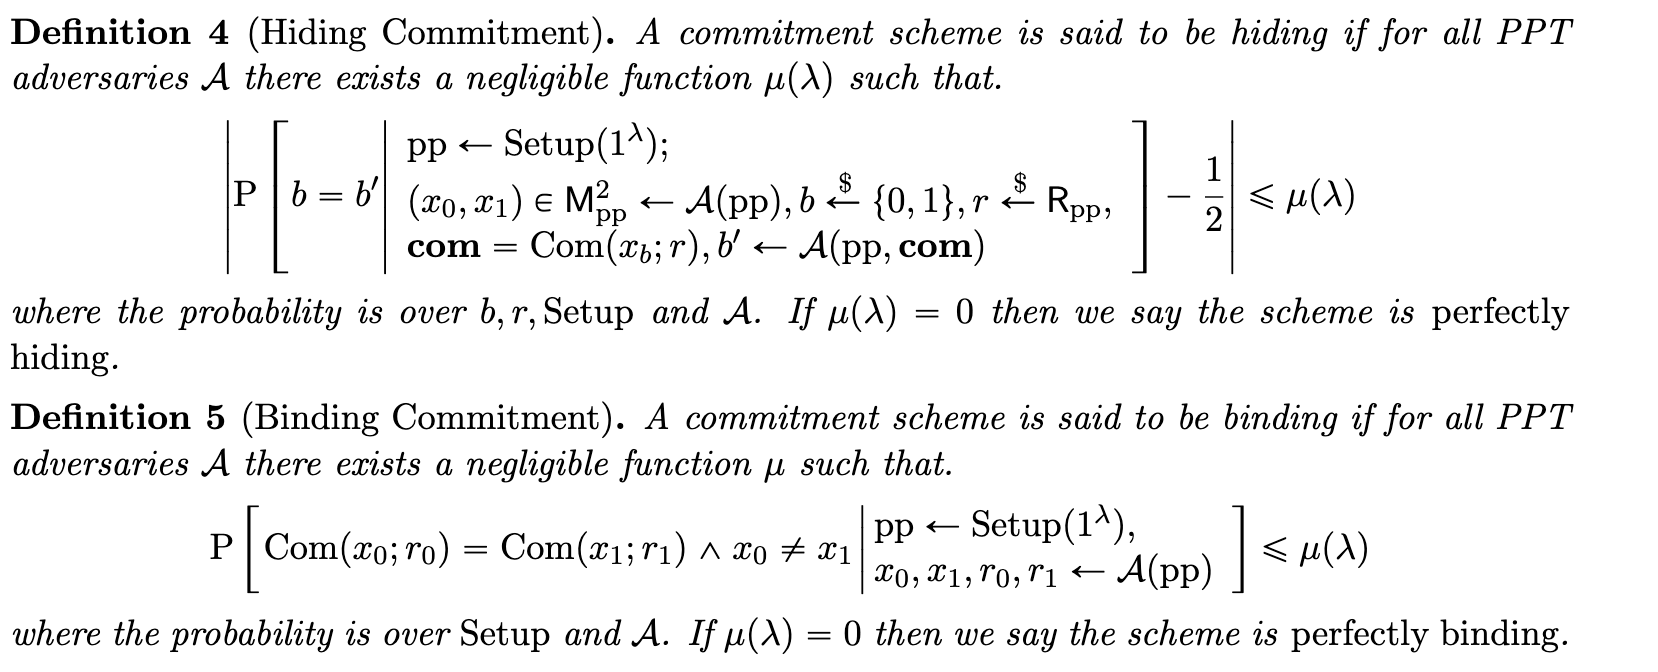
\includegraphics[width=0.8\textwidth]{images/lecture_2/bulletproof.png}
            \caption{This is not that hard as it seems. Figure from ``\textit{Bulletproofs: Short Proofs for Confidential Transactions and More}''}
            \label{fig:wuuttt}
        \end{figure}
    \end{frame}

    \section{Quick Recap}

    \begin{frame}{Quick Recap}
        \begin{enumerate}
            \item We know how to read formal statements, like 
            \begin{equation*}
                (\forall n \in \mathbb{N}) \, (\exists k \in \mathbb{Z}): \{n=2k+1 \vee n = 2k\}
            \end{equation*}
            \item Group $\mathbb{G}$ is a set with a binary operation that satisfies certain rules. In this lecture, we will use the \textbf{multiplicative} notation: for example, $g^{\alpha}$ means $g$ multiplied by itself $\alpha$ times.
            \item Probability of event $E$ is denoted by $\text{Pr}[E]$ -- we will need it further.
        \end{enumerate}
    \end{frame}

    \section{Security Analysis}

    \subsection{Cipher Definition}

    \begin{frame}{Introducing the Cipher: a bit of Formalism}
        We will consider an example of a cipher to demonstrate the notion of security.

        Let us introduce three sets:
        \begin{itemize}
            \item $\mathcal{K}$ -- a set of all possible keys.
            \item $\mathcal{M}$ -- a set of all possible messages. For example, $\mathcal{M} = \{0,1\}^n$ -- all binary strings of length $n$.
            \item $\mathcal{C}$ -- a set of all possible ciphertexts.
        \end{itemize}

        The cipher is defined over a tuple $(\mathcal{K}, \mathcal{M}, \mathcal{C})$.

        \begin{block}{Tiny Note}
            Cryptography is a very formalized field, but everything considered is well-known to you.
        \end{block}
    \end{frame}

    \begin{frame}{Introducing the Cipher}
        \begin{definition}
            Cipher scheme $\mathcal{E} = (E,D)$ over the space $(\mathcal{K}, \mathcal{M}, \mathcal{C})$ consists of two efficiently computable methods:
            \begin{itemize}
                \item $E: \mathcal{K} \times \mathcal{M} \to \mathcal{C}$ -- encryption method, that based on the provided message $m \in \mathcal{M}$ and key $k \in \mathcal{K}$ outputs the cipher $c = E(k,m) \in \mathcal{C}$.
                \item $D: \mathcal{K} \times \mathcal{C} \to \mathcal{M}$ -- decryption method, that based on the provided cipher $c \in \mathcal{C}$ and key $k \in \mathcal{K}$ outputs the message $m = D(k,c) \in \mathcal{M}$.
            \end{itemize}
        \end{definition}

        We require the \textbf{correctness}:
        \begin{equation*}
            \forall k \in \mathcal{K}, \forall m \in \mathcal{M}: D(k,E(k,m)) = m.
        \end{equation*}

        \begin{alertblock}{Question}
            What else cipher must have to be practical?
        \end{alertblock}
    \end{frame}

    \begin{frame}{Defining Security}
        Typically, the security is defined as a game between the adversary ($\mathcal{A}$) and the challenger ($\mathcal{C}h$).

        \begin{figure}
            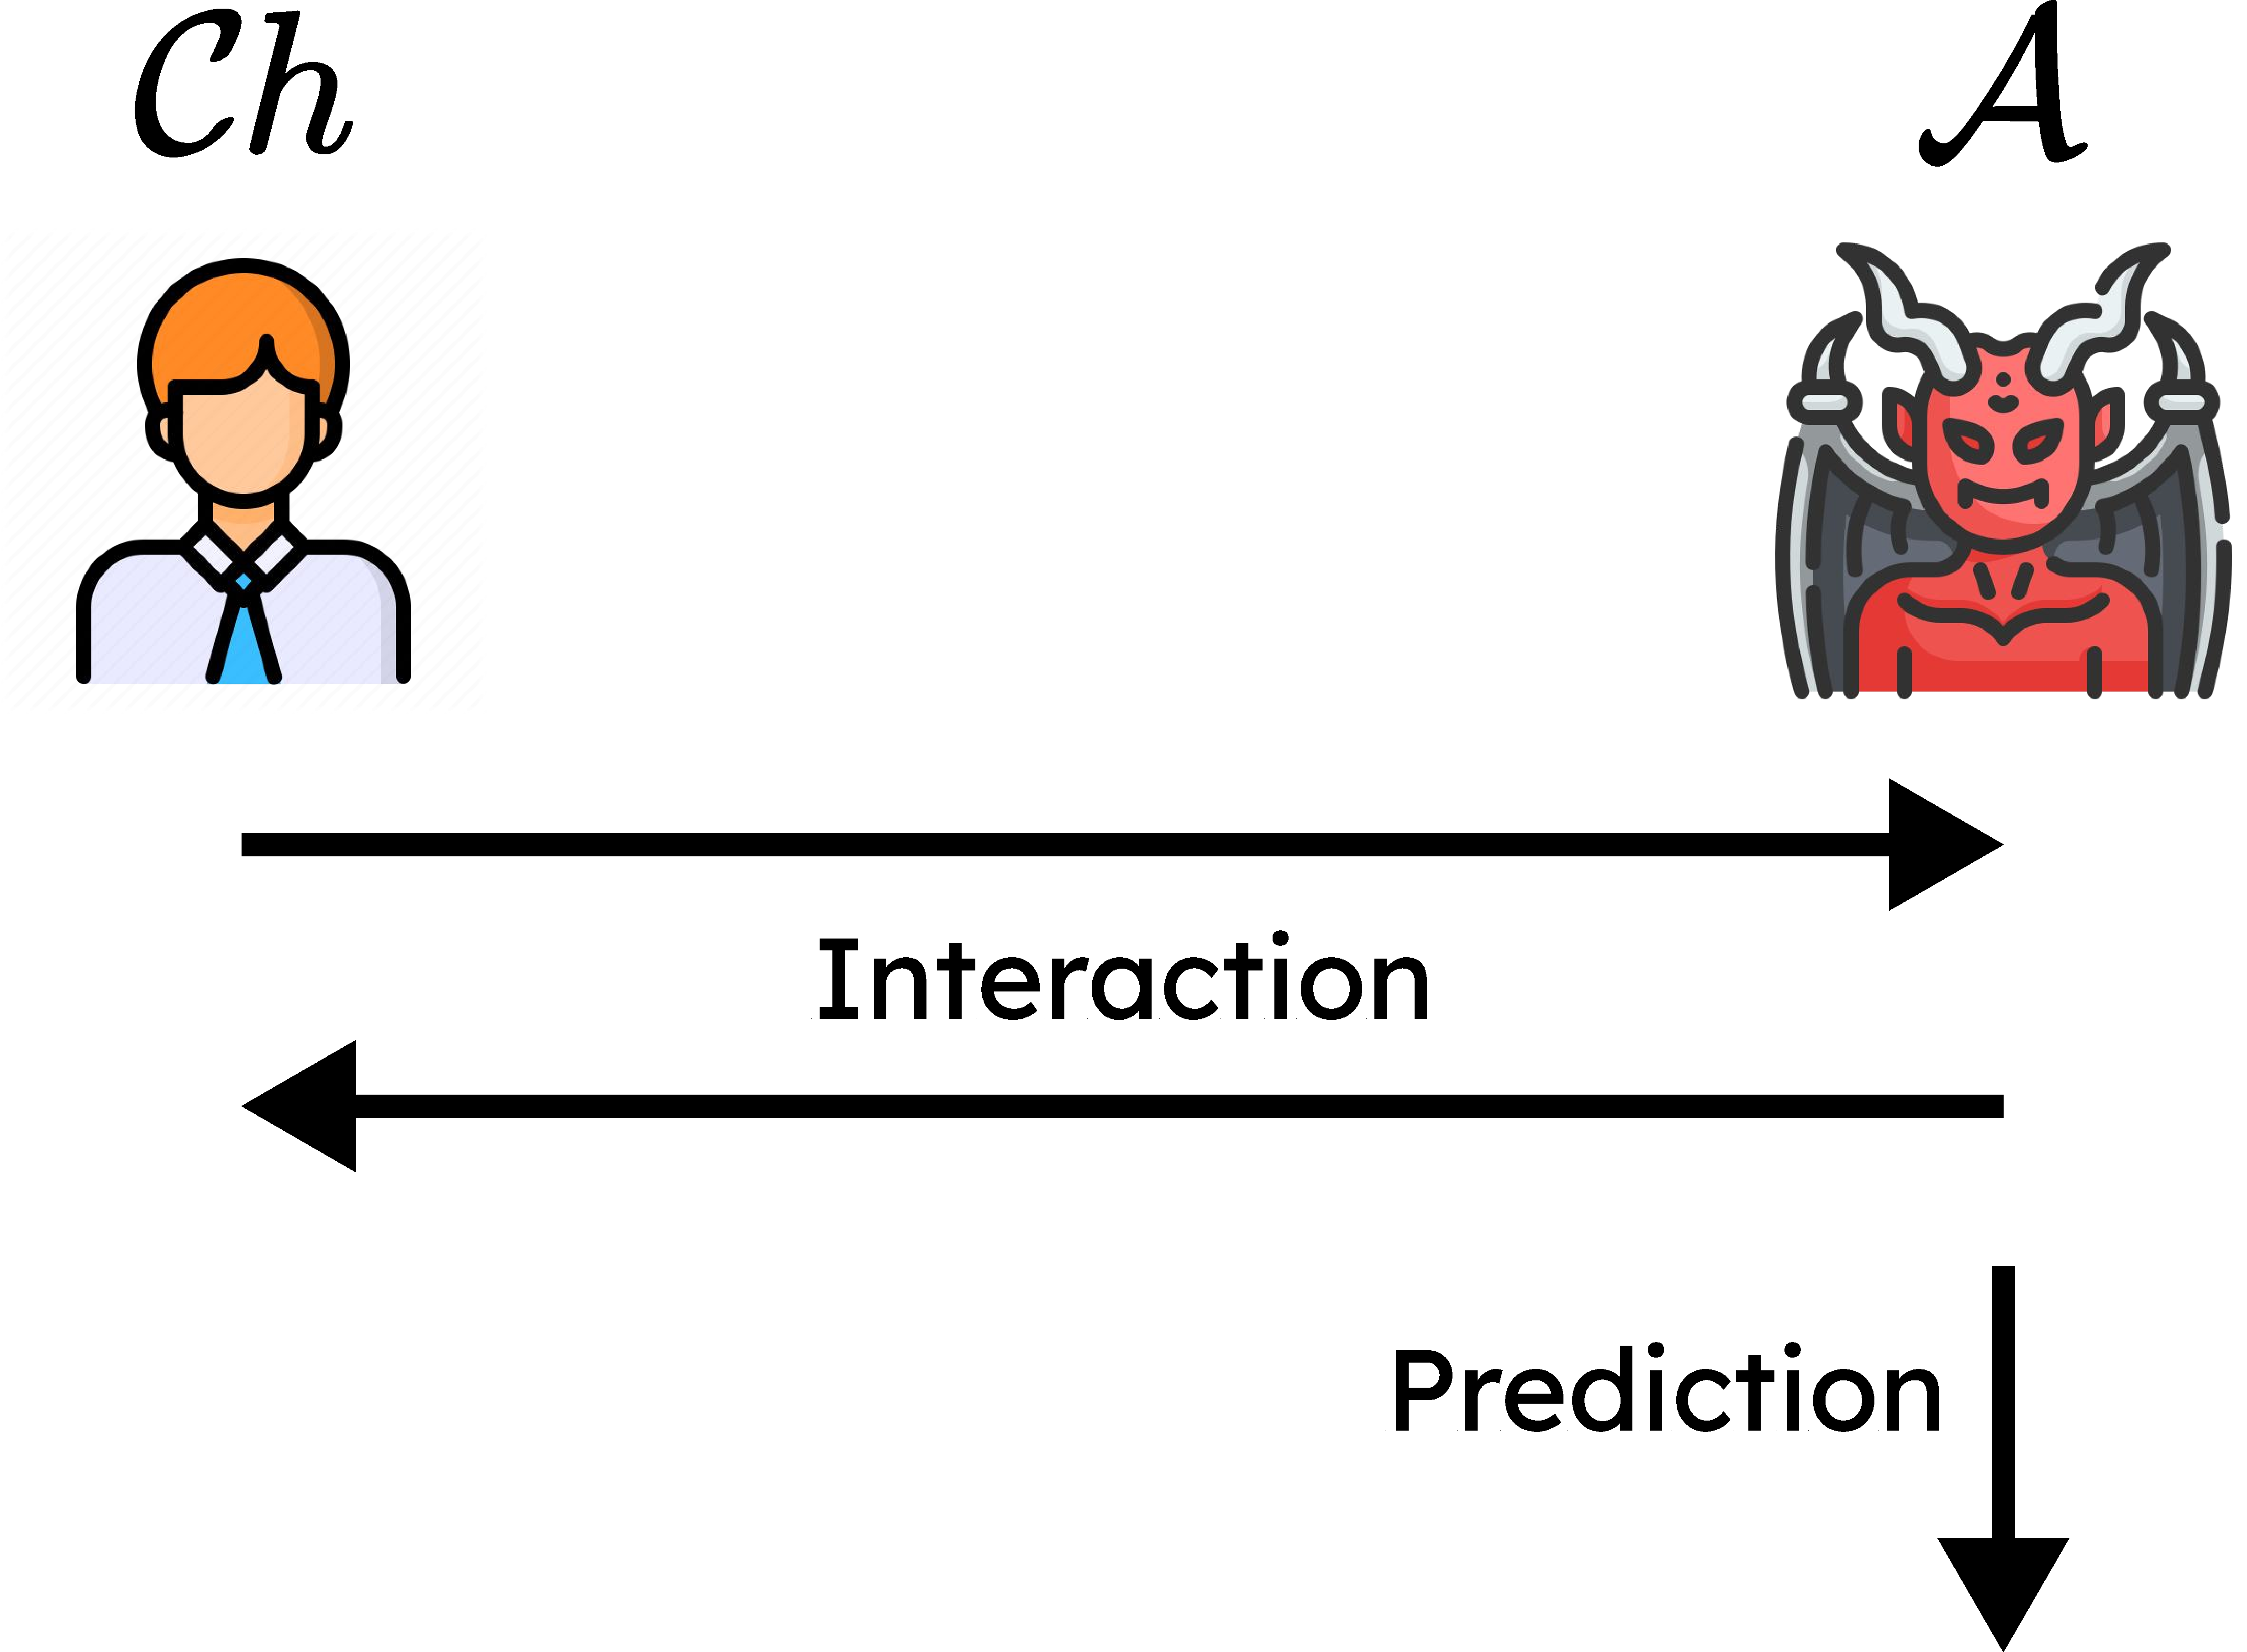
\includegraphics[width=0.6\textwidth]{images/lecture_2/interaction.pdf}
            \caption{Challenger $\mathcal{C}h$ follows a straightforward protocol, while the adversary $\mathcal{A}$ might take any strategy to win the game.}
            \label{fig:wuuttt}
        \end{figure}
    \end{frame}

    \subsection{Bit Guessing Game}
    \begin{frame}{Semantic Security: Bit Guessing Game}
        \begin{figure}
            \centering
            \begin{tikzpicture}[thick,scale=0.8, every node/.style={scale=0.8}]
                \node[inner sep=0pt, align=center] (challenger) {
\includegraphics[width=0.75cm]{../lectures/images/lecture_2/challenger.png}\\Challenger $\mathcal{C}h$};
                \node[inner sep=0pt, align=center, right=5cm of challenger] (adversary) {
\includegraphics[width=0.75cm]{../lectures/images/lecture_2/demon.png}\\Adversary $\mathcal{A}$};
        
                \draw [dashed,line width=0.3mm] ([yshift=-0.5cm]challenger.south) -- ([yshift=-7cm]challenger.south);
                \draw [dashed,line width=0.3mm] ([yshift=-0.5cm]adversary.south) -- ([yshift=-7cm]adversary.south);
        
                \draw[-{Stealth[length=3mm]},line width=0.4mm] ([yshift=-1.5cm]adversary.south) coordinate (l2)--(l2-|challenger) node[midway, above=2mm, fill=white]{Send $m_0, m_1 \in \mathcal{M}, |m_0| = |m_1|$};
        
                \node[align=center,fill=white!5,thick,below=2.5cm of challenger](challenger-actions){
                \noindent\rule{3.5cm}{0.8pt}\\
                $b \xleftarrow{R} \{0,1\}$ \\
                $k \xleftarrow{R} \mathcal{K}$ \\
                $c \gets E(k,m_b)$ \\
                \noindent\rule{3.5cm}{0.8pt}};
        
                \draw[-{Stealth[length=3mm]},line width=0.4mm] ([yshift=-6cm]challenger.south) coordinate (l2)--(l2-|adversary) node[midway, above=2mm, fill=white]{Send cipher $c$};
        
                \node[align=center,fill=white!5,thick,below=5cm of adversary](adversary-guess){
                \noindent\rule{3.5cm}{0.8pt}\\
                Guess bit $\hat{b} \in \{0,1\}$\\
                \noindent\rule{3.5cm}{0.8pt}};
            \end{tikzpicture}
        \end{figure}
    \end{frame}

    \begin{frame}{Semantic Security: Bit Guessing Game}

        \begin{alertblock}{Question \#1}
            Suppose our cipher is perfect. What is the probability that the adversary guesses the bit $b$ correctly? (that is, $b = \hat{b}$)
        \end{alertblock}

        \begin{definition}
            \textbf{Advantage in the Cipher Big Guessing Game} of the adversary $\mathcal{A}$ given cipher $\mathcal{E}$ is defined as:
            \begin{equation*}
                \text{SS}\mathsf{adv}[\mathcal{E}, \mathcal{A}] := \left| \Pr[\hat{b} = b] - \frac{1}{2} \right|
            \end{equation*}
        \end{definition}

        \begin{definition}
            The cipher $\mathcal{E}$ is called \textbf{semantically secure} if for any adversary $\mathcal{A}$ the advantage $\text{SS}\mathsf{adv}[\mathcal{E}, \mathcal{A}]$ is \textbf{negligible}.
        \end{definition}
    \end{frame}

    \begin{frame}{Advantage}
        \begin{alertblock}{Question \#2}
            If adversary can guess the bit with probability $0.000000001$, is the cipher semantically secure?
        \end{alertblock}

        \begin{alertblock}{Question \#3}
            If adversary has the advantage $0.0001$, is the cipher semantically secure?
        \end{alertblock}

        \begin{block}{Note}
            Advantage is just a measure of how many information is leaked to the adversary. The smaller the advantage, the better the cryptographic system. Formally, we want advantage to be \textbf{negligible}.
        \end{block}

        But what does it mean to be \textbf{negligible}?
    
    \end{frame}

    \subsection{Neglibility}

    \begin{frame}{Neglibility}
        \textbf{In practice}, neglibible means below $2^{-128}$ (called $128$ bits of security).

        In theory, however\ldots

        \begin{definition}
            \textbf{Security parameter}, denoted by $\lambda \in \mathbb{N}$, is just a variable that measures the input size of some computational program.
        \end{definition}

        \begin{example}
            The security of the group of points on the elliptic curve (say, $\mathbb{G}$) is defined by the number of bits in the order of the group. So if $|\mathbb{G}|$ is $256$ bits long, then we can define $\lambda = 256$.
        \end{example}
    \end{frame}

    \begin{frame}{Neglible Functions}
        Now, the probability of advesary winning the game depends on $\lambda$ and we want this dependence to decrease rapidly.

        \begin{definition}
            A function $f: \mathbb{N} \to \mathbb{R}$ is called \textbf{negligible} if for all $c \in \mathbb{R}_{>0}$ there exists $n_c \in \mathbb{N}$ such that for any $n \geq n_c$ we have $|f(n)| < 1/n^c$.
        \end{definition}
        
        The alternative definition, which is problably easier to interpret, is the following.
        
        \begin{theorem}
            A function $f: \mathbb{N} \to \mathbb{R}$ is \textbf{negligible} if and only if for any $c \in \mathbb{R}_{>0}$, we have
            \begin{equation*}
                \lim_{n \to \infty} f(n)n^c = 0
            \end{equation*}
        \end{theorem}
    \end{frame}

    \begin{frame}{Neglible Functions Examples}
        \begin{example}
            The function $f(\lambda) = 2^{-\lambda}$ is negligible since for any $c \in \mathbb{R}_{>0}$ we have $\lim_{\lambda \to \infty} 2^{-\lambda}\lambda^c = 0$.
        
            The function $g(\lambda) = \frac{1}{\lambda!}$ is also negligible for similar reasons.
        \end{example}
        
        \begin{example}
            The function $h(\lambda) = \frac{1}{\lambda}$ is not negligible since for $c = 1$ we have
            \begin{equation*}
                \lim_{\lambda \to \infty} \frac{1}{\lambda} \times \lambda = 1 \neq 0
            \end{equation*}
        \end{example}

        \begin{alertblock}{Question}
            Is the function $u(\lambda) = \lambda^{-10000}$ negligible?
        \end{alertblock}
    \end{frame}

    \subsection{Other Examples}
    \begin{frame}{Discrete Logarithm Problem (DL)}
        \begin{definition}
            Assume that $\mathbb{G}$ is a cyclic group of prime order $r$ generated by $g \in \mathbb{G}$. Define the following game:
            \begin{enumerate}
                \item Both challenger $\mathcal{C}h$ and adversary $\mathcal{A}$ take a description $\mathbb{G}$ as an input: order $r$ and generator $g \in \mathbb{G}$.
                \item $\mathcal{C}h$ computes $\alpha \xleftarrow{R} \mathbb{Z}_r, u \gets g^{\alpha}$ and sends $u \in \mathbb{G}$ to $\mathcal{A}$.
                \item The adversary $\mathcal{A}$ outputs $\hat{\alpha} \in \mathbb{Z}_r$.
            \end{enumerate}
        
            We define $\mathcal{A}$'s \textbf{advantage in solving the discrete logarithm problem in $\mathbb{G}$}, denoted as $\text{DL}\mathsf{adv}[\mathcal{A},\mathbb{G}]$, as the probability that $\hat{\alpha} = \alpha$.
        \end{definition}
        
        \begin{definition}
            The \textbf{Discrete Logarithm Assumption} holds in the group $\mathbb{G}$ if for any efficient adversary $\mathcal{A}$ the advantage $\text{DL}\mathsf{adv}[\mathcal{A},\mathbb{G}] \leq \text{negl}(\lambda)$.
        \end{definition}
    \end{frame}

    \begin{frame}{Computational Diffie-Hellman Assumption (CDH)}
        \begin{definition}
            Let $\mathbb{G}$ be a cyclic group of prime order $r$ generated by $g \in \mathbb{G}$. Define the following game:
            \begin{enumerate}
                \item $\mathcal{C}h$ computes $\alpha, \beta \xleftarrow{R} \mathbb{Z}_r, u \gets g^{\alpha}, v \gets g^{\beta}, w \gets g^{\alpha\beta}$ and sends $u,v \in \mathbb{G}$ to $\mathcal{A}$.
                \item The adversary $\mathcal{A}$ outputs $\hat{w} \in \mathbb{G}$.
            \end{enumerate}
        
            We define $\mathcal{A}$'s \textbf{advantage in solving the computational Diffie-Hellman problem in $\mathbb{G}$}, denoted as $\text{CDH}\mathsf{adv}[\mathcal{A},\mathbb{G}]$, as the probability that $\hat{w} = w$.
        \end{definition}
        
        \begin{definition}
            The \textbf{Computational Diffie-Hellman Assumption} holds in the group $\mathbb{G}$ if for any efficient adversary $\mathcal{A}$ the advantage $\text{CDH}\mathsf{adv}[\mathcal{A},\mathbb{G}]$ is negligible.
        \end{definition}
    \end{frame}

    \begin{frame}{Decisional Diffie-Hellman Assumption (DDH)}
        \begin{definition}
            Let $\mathbb{G}$ be a cyclic group of prime order $r$ generated by $g \in \mathbb{G}$. Define the following game:
            \begin{enumerate}
                \item $\mathcal{C}h$ computes $\alpha, \beta,\gamma \xleftarrow{R} \mathbb{Z}_r, u \gets g^{\alpha}, v \gets g^{\beta}, w_0 \gets g^{\alpha\beta}, w_1 \gets g^{\gamma}$. Then, $\mathcal{C}h$ flips a coin $b \xleftarrow{R} \{0,1\}$ and sends $(u,v,w_b)$ to $\mathcal{A}$.
                \item The adversary $\mathcal{A}$ outputs the predicted bit $\hat{b} \in \{0,1\}$.
            \end{enumerate}
        
            We define $\mathcal{A}$'s \textbf{advantage in solving the Decisional Diffie-Hellman problem in $\mathbb{G}$}, denoted as $\text{DDH}\mathsf{adv}[\mathcal{A},\mathbb{G}]$, as
            \begin{equation*}
                \text{DDH}\mathsf{adv}[\mathcal{A},\mathbb{G}] := \left| \Pr[b = \hat{b}] - \frac{1}{2} \right|
            \end{equation*}
        \end{definition}

        Let us show when DDH does not hold!
    \end{frame}

    \begin{frame}{Even-ordered Cyclic Group}
        \begin{theorem}
            Suppose that $\mathbb{G}$ is a cyclic group of an even order. Then, the Decision
            Diffie-Hellman Assumption does not hold in $\mathbb{G}$. In fact, there is an efficient adversary $\mathcal{A}$ with an advantage $1/4$.
        \end{theorem}

        \textbf{Idea of proof.} We first prove the following statement:

        \begin{lemma}
            Based on $u = g^{\alpha} \in \mathbb{G}$, it is possible to determine the parity of $\alpha$.
        \end{lemma}

        \textbf{Lemma proof.} Notice that if $\alpha=2\alpha'$, then
        \begin{equation*}
            u^n = g^{\alpha n} = g^{2\alpha' n} = (g^{2n})^{\alpha'} = 1^{\alpha'} = 1
        \end{equation*}

        Therefore, if $u = g^{\alpha}, v = g^{\beta}, w = g^{\gamma}$, adversary knows the parity of $\alpha, \beta, \gamma$. He then checks if parity of $\alpha\beta$ equals parity of $\gamma$.
    \end{frame}

    \section{Polynomials}

    \subsection{Definition}

    \begin{frame}{Definition}
      \begin{definition}
        A \textbf{polynomial} $f(x)$ is a function of the form
        \begin{equation*}
            p(x) = c_0 + c_1 x + c_2 x^2 + \cdots + c_n x^n = \sum_{k=0}^{n} c_k x^k,
        \end{equation*}
        where $c_0, c_1, \dots, c_n$ are coefficients of the polynomial.
    \end{definition}
    
    \begin{definition}
        A set of polynomials depending on $x$ with coefficients in a field $\mathbb{F}$ is denoted as $\mathbb{F}[x]$, that is
        \begin{equation*}
            \mathbb{F}[x] = \left\{p(x) = \sum_{k=0}^{n} c_k x^k: c_k \in \mathbb{F}, \; k = 0,\dots,n\right\}.
        \end{equation*}
    \end{definition}
    \end{frame}

    \begin{frame}{Examples of Polynomials}
      \begin{example}
        Consider the finite field $\mathbb{F}_3$. Then, some examples of polynomials from $\mathbb{F}_3[x]$ are listed below:
        \begin{enumerate}
            \item $p(x) = 1 + x + 2x^2$.
            \item $q(x) = 1 + x^2 + x^3$.
            \item $r(x) = 2x^3$.
        \end{enumerate}
    
       If we were to evaluate these polynomials at $1 \in \mathbb{F}_3$, we would get:
        \begin{enumerate}
            \item $p(1) = 1 + 1 + 2 \cdot 1 \; \text{mod} \; 3 = 1$.
            \item $q(1) = 1 + 1 + 1 \; \text{mod} \; 3 = 0$.
            \item $r(1) = 2 \cdot 1 = 2$.
        \end{enumerate}
    \end{example}
    \end{frame}    

    \begin{frame}{More about polynomials}
      \begin{definition}
          The \textbf{degree} of a polynomial $p(x) = c_0+c_1x+c_2x^2+\dots$ is the largest $k \in \mathbb{Z}_{\geq 0}$ such that $c_k \neq 0$. We denote the degree of a polynomial as $\deg p$. We also denote by $\mathbb{F}^{(\leq m)}[x]$ a set of polynomials of degree at most $m$.
      \end{definition}
      
      \begin{example}
          The degree of the polynomial $p(x) = 1 + 2x + 3x^2$ is $2$, so $p(x) \in \mathbb{F}_3^{(\leq 2)}[x]$.
      \end{example}
      
      \begin{theorem}
          For any two polynomials $p,q \in \mathbb{F}[x]$ and $n = \deg p, m = \deg q$, the following two statements are true:
          \begin{enumerate}
              \item $\deg (pq) = n + m$.
              \item $\deg (p + q) = \max\{n,m\}$ if $n \neq m$ and $\deg (p+q) \leq m$ for $m=n$.
          \end{enumerate}
      \end{theorem}
    \end{frame}
    \subsection{Roots and Divisibility}
    \begin{frame}{Roots of Polynomials}
      \begin{definition}
          Let $p(x) \in \mathbb{F}[x]$ be a polynomial of degree $\deg p \geq 1$. A field element $x_0 \in \mathbb{F}$ is called a root of $p(x)$ if $p(x_0) = 0$.
      \end{definition}
      
      \begin{example}
          Consider the polynomial $p(x) = 1 + x + x^2 \in \mathbb{F}_3[x]$. Then, $x_0=1$ is a root of $p(x)$ since $p(x_0) = 1 + 1 + 1 \; \text{mod} \; 3 = 0$.
      \end{example}

      \begin{theorem}
        Let $p(x) \in \mathbb{F}[x], \deg p \geq 1$. Then, $x_0 \in \mathbb{F}$ is a root of $p(x)$ if and only if there exists a polynomial $q(x)$ (with $\deg q = n-1$) such that
        \begin{equation*}
            p(x) = (x-x_0)q(x)
        \end{equation*}
    \end{theorem}
    \end{frame}
    \begin{frame}{Polynomial Division}
      \begin{theorem}
        Given $f,g \in \mathbb{F}[x]$ with $g \neq 0$, there are unique polynomials $p,q \in \mathbb{F}[x]$ such that 
        \begin{equation*}
            f = q \cdot g + r, \; 0 \leq \deg r < \deg g
        \end{equation*}
    \end{theorem}
    
    \begin{example}
        Consider $f(x) = x^3+2$ and $g(x) = x+1$ over $\mathbb{R}$. Then, we can write $f(x) = (x^2-x+1)g(x) + 1$, so the remainder of the division is $r \equiv 1$. Typically, we denote this as:
        \begin{equation*}
            f \, \text{div} \, g = x^2-x+1, \quad f \, \text{mod} \, g = 1.
        \end{equation*}
    
        The notation is pretty similar to one used in integer division.
    \end{example}
    \end{frame}

    \begin{frame}{Polynomial Divisibility}
      \begin{definition}
        A polynomial $f(x) \in \mathbb{F}[x]$ is called \textbf{divisible} by $g(x) \in \mathbb{F}[x]$ (or, $g$ \textbf{divides} $f$, written as $g \mid f$) if there exists a polynomial $h(x) \in \mathbb{F}[x]$ such that $f=gh$.
    \end{definition}
    
    \begin{theorem}
        If $x_0 \in \mathbb{F}$ is a root of $p(x) \in \mathbb{F}[x]$, then $(x-x_0) \mid p(x)$.
    \end{theorem}
    
    \begin{definition}
        A polynomial $f(x) \in \mathbb{F}[x]$ is said to be \textbf{irreducible} in $\mathbb{F}$ if there are no polynomials $g,h \in \mathbb{F}[x]$ both of degree more than $1$ such that $f = gh$.
    \end{definition}
    \end{frame}

    \begin{frame}{Polynomial Divisibility}
      \begin{example}
        A polynomial $f(x) = x^2+16$ is irreducible in $\mathbb{R}$. Also $f(x) = x^2-2$ is irreducible over $\mathbb{Q}$, yet it is reducible over $\mathbb{R}$: $f(x) = (x-\sqrt{2})(x+\sqrt{2})$. 
    \end{example}
    
    \begin{example}
        There are no polynomials over complex numbers $\mathbb{C}$ with degree more than $2$ that are irreducible. This follows from the \textit{fundamental theorem of algebra}. For example, $x^2+16 = (x-4i)(x+4i)$.
    \end{example}
    \end{frame}
    \subsection{Interpolation}
    \begin{frame}{Interpolation}
      \begin{alertblock}{Question}
        How can we define the polynomial?
      \end{alertblock}

      The most obvious way is to specify coefficients $(c_0,c_1,\dots,c_n)$. Can we do it in a different way?

      \begin{theorem}
        Given $n+1$ distinct points $(x_0,y_0),\dots,(x_n,y_n)$, there exists a unique polynomial $p(x)$ of degree at most $n$ such that $p(x_i) = y_i$ for all $i=0,\dots,n$.
      \end{theorem}
    \end{frame}

    \begin{frame}{Illustration with two points}
      \begin{figure}
        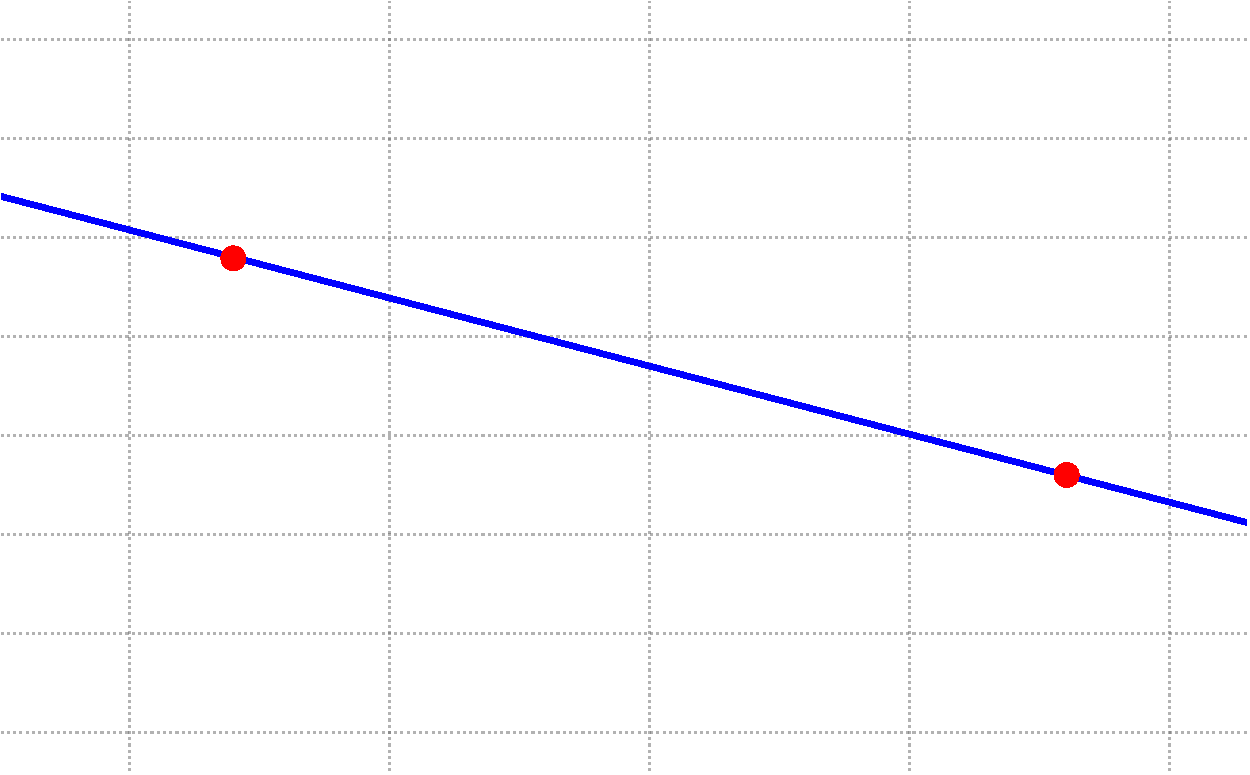
\includegraphics[width=0.8\textwidth]{images/lecture_1/simple_interpolation.pdf}
        \caption{$2$ points on the plane uniquely define the polynomial of degree $1$ (linear function).}
        \label{fig:simple_interpolation}
      \end{figure}
    \end{frame}

    \begin{frame}{Illustration with five points}
      \begin{figure}
        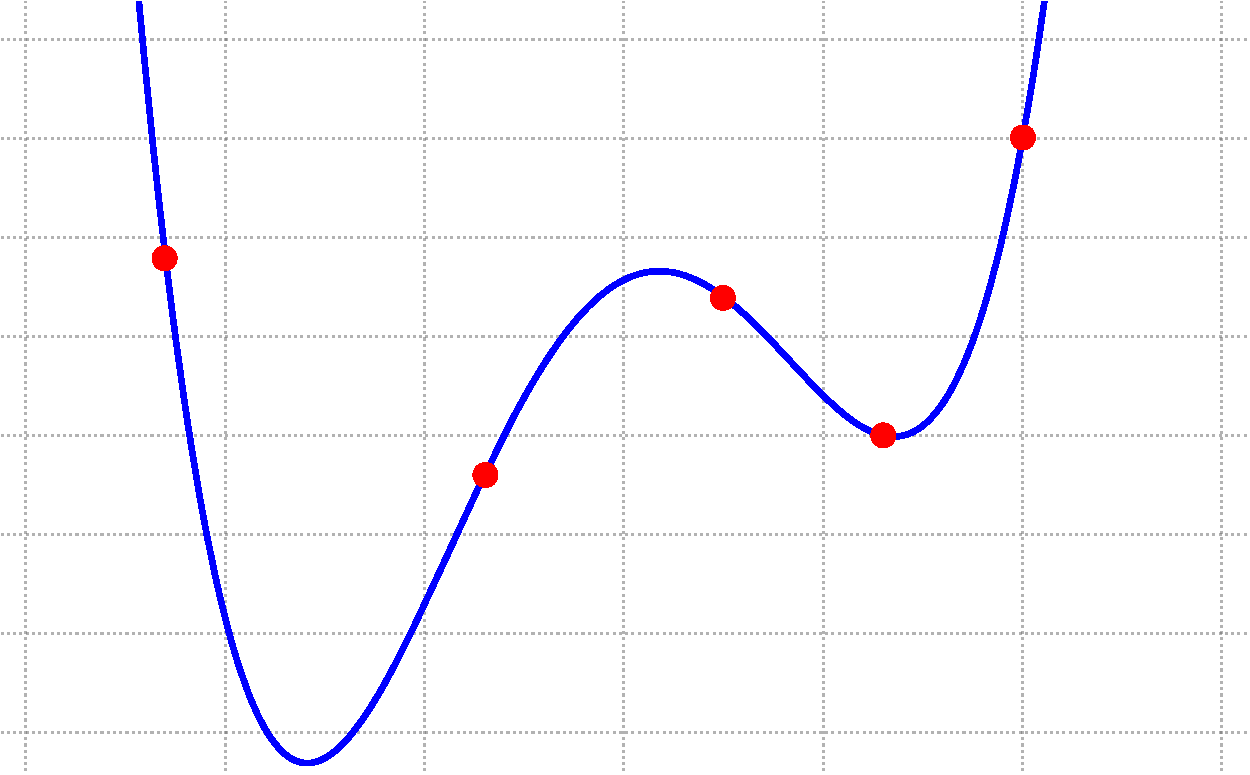
\includegraphics[width=0.8\textwidth]{images/lecture_1/interpolation.pdf}
        \caption{$5$ points on the plane uniquely define the polynomial of degree $4$.}
        \label{fig:interpolation}
      \end{figure}
    \end{frame}

    \begin{frame}{Illustration with three points}
      \begin{figure}
        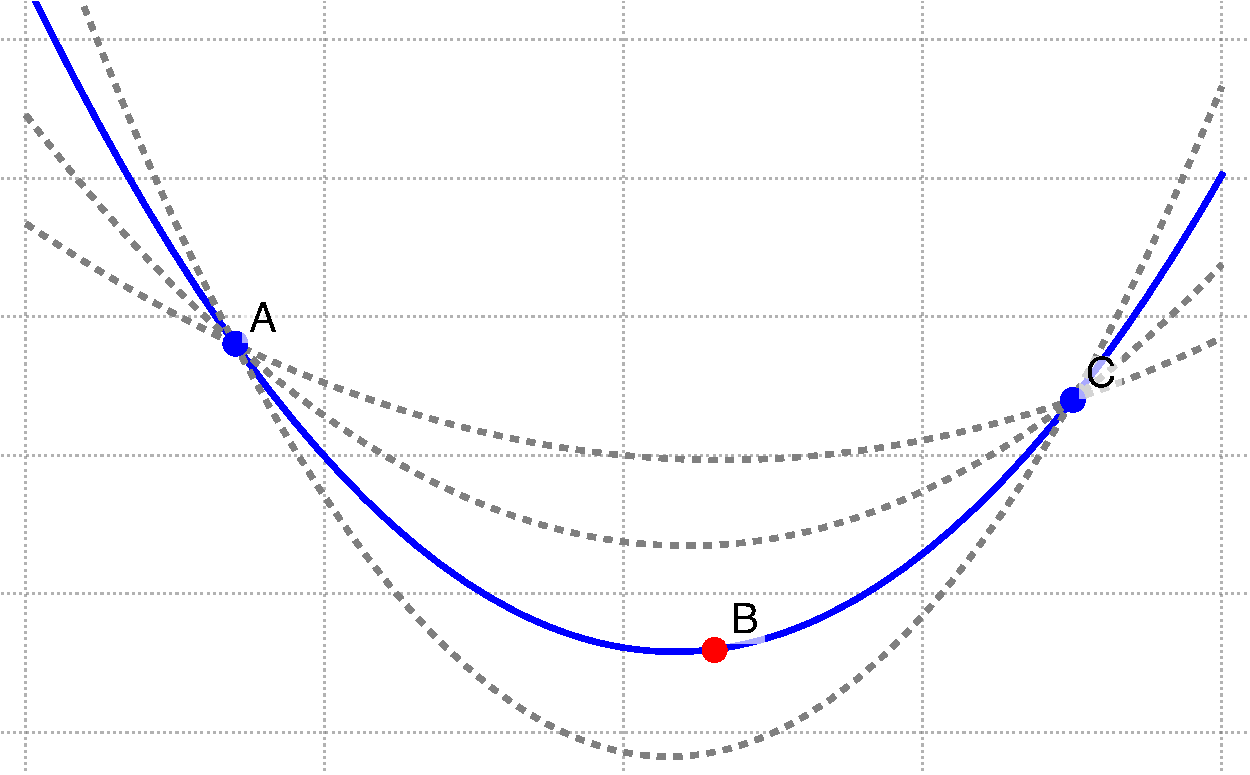
\includegraphics[width=0.8\textwidth]{images/lecture_1/shamir_demo.pdf}
        \caption{$2$ points are not enough to define the quadratic polynomial ($c_2x^2+c_1x+c_0$).}
        \label{fig:interpolation}
      \end{figure}
    \end{frame}

    \begin{frame}{Lagrange Interpolation}
      One of the ways to interpolate the polynomial is to use the Lagrange interpolation.

      \begin{theorem}
        Given $n+1$ distinct points $(x_0,y_0),\dots,(x_n,y_n)$, the polynomial $p(x)$ that passes through these points is given by
        \begin{equation*}
            p(x) = \sum_{i=0}^{n} y_i \ell_i(x), \quad \ell_i(x) = \prod_{i=0, j \neq i}^n \frac{x-x_j}{x_i-x_j}.
        \end{equation*}
    \end{theorem}
    \end{frame}

    \subsection{Interpolation Applications: Shamir Secret Sharing}
    \begin{frame}{Application: Shamir Secret Sharing}
      \begin{alertblock}{Motivation}    
        How to share a secret $\alpha$ among $n$ people in such a way that any $t$ of them can reconstruct the secret, but any $t-1$ cannot?
      \end{alertblock}  

      \begin{definition}
        \textbf{Secret Sharing} scheme is a pair of efficient algorithms $(\mathsf{Gen}, \mathsf{Comb})$ which work as follows:
        \begin{itemize}
            \item $\mathsf{Gen}(\alpha, t, n)$: probabilistic sharing algorithm that yields $n$ shards $(\alpha_1,\dots,\alpha_t)$ for which $t$ shards are needed to reconstruct the secret $\alpha$.
            \item $\mathsf{Comb}(\mathcal{I}, \{\alpha_i\}_{i \in \mathcal{I}})$: deterministic reconstruction algorithm that reconstructs the secret $\alpha$ from the shards $\mathcal{I} \subset \{1,\dots,n\}$ of size $t$.
        \end{itemize}
    \end{definition}
    \end{frame}

    \begin{frame}{Shamir's Protocol}
      \begin{block}{Note}
        Here, we require the \textbf{correctness}: for every $\alpha \in F$, for every possible output $(\alpha_1,\dots,\alpha_n) \gets \mathsf{Gen}(\alpha, t, n)$, and any $t$-size subset $\mathcal{I}$ of $\{1,\dots,n\}$ we have
        \begin{equation}
            \mathsf{Comb}(\mathcal{I}, \{\alpha_i\}_{i \in \mathcal{I}}) = \alpha.
        \end{equation}
      \end{block}

      \begin{definition}
        Now, \textbf{Shamir's protocol} works as follows: $F=\mathbb{F}_q$ and
        \begin{itemize}
            \item $\mathsf{Gen}(\alpha, k, n)$: choose random $k_1,\dots,k_{t-1} \xleftarrow[]{R} \mathbb{F}_q$ and define the polynomial
            \begin{equation}
                \omega(x) := \alpha + k_1x + k_2x^2 + \cdots + k_{t-1}x^{t-1} \in \mathbb{F}_q^{\leq (t-1)}[x],     
            \end{equation}
            and then compute $\alpha_i \gets \omega(i) \in \mathbb{F}_q, \; i = 1,\dots,n$. 
        \end{itemize}
      \end{definition}
    \end{frame}
  
    \begin{frame}{Shamir's Protocol}
      \begin{definition}
        \begin{itemize}
            \item $\mathsf{Comb}(\mathcal{I}, \{\alpha_i\}_{i \in \mathcal{I}})$: interpolate the polynomial $\omega(x)$ using the Lagrange interpolation and output $\omega(0) = \alpha$.
        \end{itemize}
      \end{definition}

      \begin{figure}
        \centering
        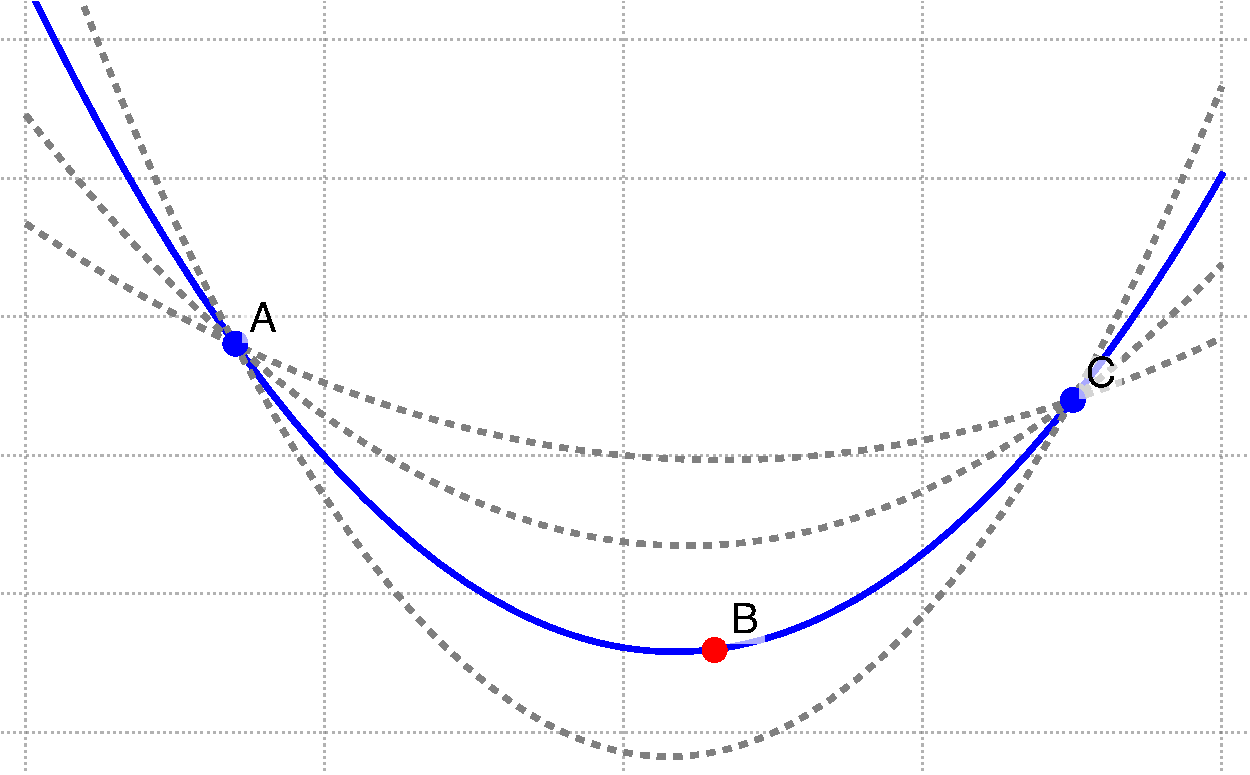
\includegraphics[width=0.5\textwidth]{images/lecture_1/shamir_demo.pdf}
        \caption{There are infinitely many quadratic polynomials passing through two \textcolor{blue}{blue} points (\textcolor{gray}{gray dashed} lines). However, knowing the \textcolor{red}{red} point allows us to uniquely determine the polynomial and thus get its value at $0$.}
        \label{fig:shamir}
      \end{figure}
    \end{frame}

    \begin{frame}{Reed-Solomon Codes}
        \begin{definition}
            \begin{itemize}
                \item Reed-Solomon codes is an error-correcting algorithm based on polynomials. It allows to restore lost or corrupted data, implement threshold secret sharing and it is used in some ZK protocols.
            \end{itemize}
          \end{definition}
  
        \begin{figure}
          \centering
          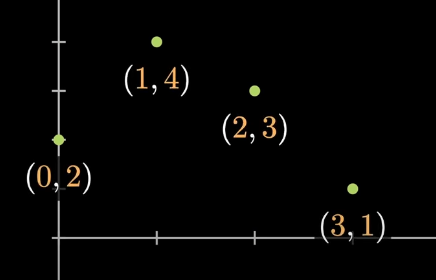
\includegraphics[width=0.5\textwidth]{images/lecture_2/reed-solomon-1.png}
          \caption{Polynomial with degree $n$ can be uniquely defined using $(n+1)$ unique points. Defining more points on the same polynomial adds a redundancy, which can be used to restore the polynomial even if some points are missing.}
          \label{fig:reed-1}
        \end{figure}
    \end{frame}

    \begin{frame}{Reed-Solomon Codes}
        The error-correcting ability of a Reed-Solomon code is $n-k$, the measure of redundancy in the block. 
        If the locations of the error symbols are not known in advance, then a Reed-Solomon code can correct up to
        $n-k/2$ erroneous symbols.
  
        \begin{figure}
          \centering
          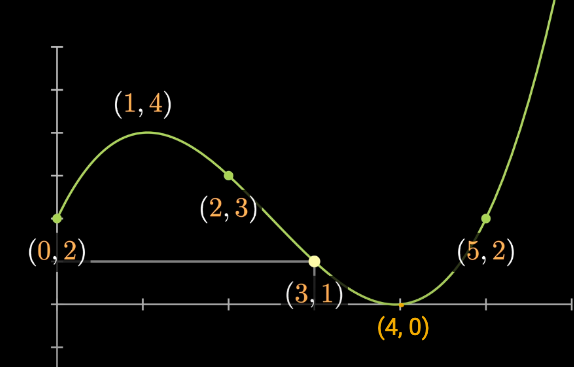
\includegraphics[width=0.5\textwidth]{images/lecture_2/reed-solomon-2.png}
          \caption{Polynomial with degree $n$ can be uniquely defined using $(n+1)$ unique points. Defining more points on the same polynomial adds a redundancy, which can be used to restore the polynomial even if some points are missing.}
          \label{fig:reed-2}
        \end{figure}
    \end{frame}


    \begin{frame}{Schwartz-Zippel Lemma}
        \begin{definition}
        Let $\mathbb{F}$ be a field. Let $f(x_1, x_2, ..., x_n)$ be a polynomial of total degree $d$. Suppose that $f$ is not the zero polynomial. Let $S$ be
        a finite subset of $\mathbb{F}$. Let $r_1, r_2, ... r_n$ be chosen at random uniformly and independently from $S$. Then the probability that 
        $f(r_1, r_2, ..., r_n) = 0$ is $\le \frac{d}{|S|}$.
        \end{definition}
  
        \begin{figure}
          \centering
          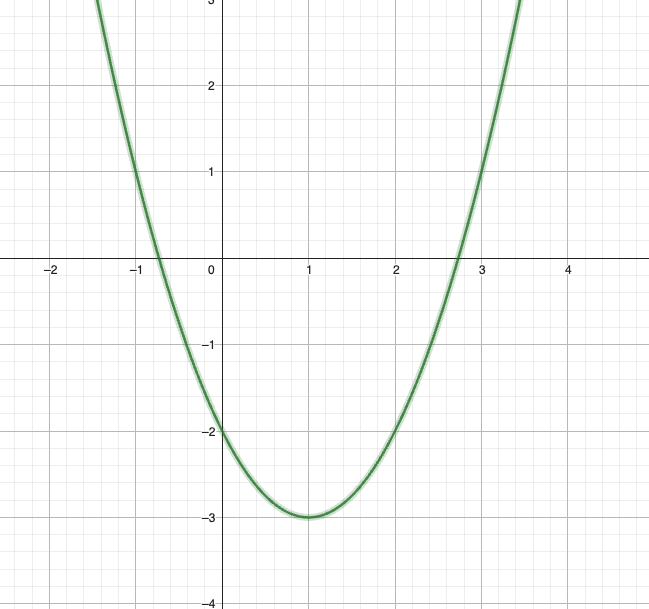
\includegraphics[width=0.5\textwidth]{images/lecture_2/Schwartz-Zippel-1.png}
          \caption{Schwartz-Zippel Lemma. Polynomial}
          \label{fig:schwartz-1}
        \end{figure}
    \end{frame}

    \begin{frame}{Schwartz-Zippel Lemma}
        \begin{definition}
            Let $F = \mathbb{F}_3$, $f(x) = x^2 - 5x + 6$, $S = F$, $r \xleftarrow{R} \mathbb{F}_3$.
            Schwartz-Zippel lemma says that the probability that $f(r) = 0$ is $\le \frac{2}{3}$.
        \end{definition}
  
        \begin{figure}
          \centering
          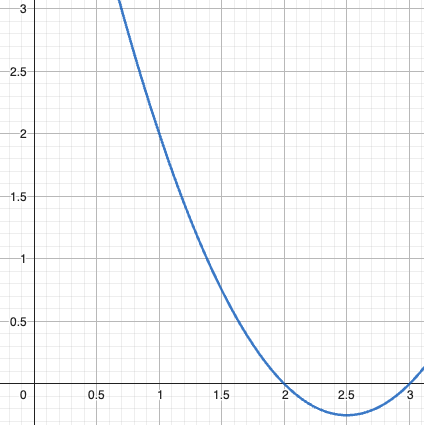
\includegraphics[width=0.5\textwidth]{images/lecture_2/Schwartz-Zippel-2.png}
          \caption{Schwartz-Zippel Lemma. Polynomial}
          \label{fig:schwartz-2}
        \end{figure}
    \end{frame}

    \begin{frame}{Schwartz-Zippel Lemma}
        Given two polynomials $P, Q$ with  degree $d$ in a field $\mathbb{F}_p$, for $r \xleftarrow{R} \mathbb{F}_3$: $\Pr[P(r) == Q(r)] \le \frac{d}{p}$.
        For large fields, where  $\frac{d}{p}$ is negligible, this property allows to succinctly check the equality of polynomials.

    \begin{proof}
        Let $H(x) := P(x) - Q(x)$. Than for each $P(x) = Q(x) \rightarrow H(x) = 0$. Applying Schwartz-Zippel lemma, the probability of $H(x) = 0$ for $x \xleftarrow{R} \mathbb{F} $ is $\le \frac{d}{|S|}$.
    \end{proof}
        
    \end{frame}

    \section{Basic Number Theory}

    \begin{frame}{Primes}
        Primes are often used when doing almost any cryptographic computation. A prime number is a natural number ($\mathbb{N}$) that is not a product
        of two smaller natural number. In other words, the prime number is divisible only by itself and 1. The first primes are: 2, 3, 5, 7, 11...
        
    \end{frame}

    \begin{frame}{Deterministic prime tests}
        A primality test is deterministic if it outputs $\mathtt{True}$ when the number is a prime and $\mathtt{False}$ when the input is composite with probability 1.
        Here is an example implementation in Rust: 

        \centering
        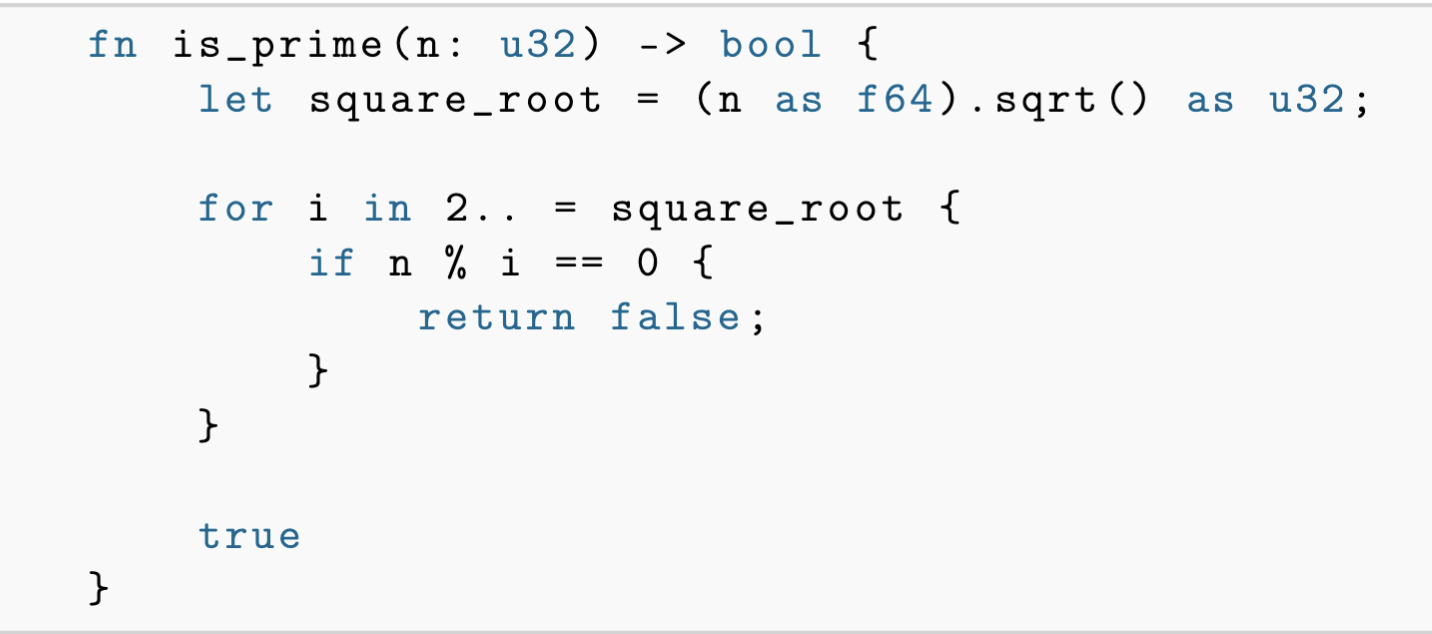
\includegraphics[width=0.8\textwidth]{images/lecture_2/prime-test-det.png}
    \end{frame}


    \begin{frame}{Probabilistic prime tests}
        A primality test is probabilistic if it outputs $\mathtt{True}$ when the number is a prime and $\mathtt{False}$ when the input is composite with probability less than 1.
        Fermat Primality and Miller-Rabin Primality Tests are examples of probabilistic primality test. 

        \begin{theorem}
            Let $p$ be a prime number and $a$ be an integer not divisible by $p$. Then $a ^ {p-1} - 1$ is always divisible by $p$:  $a^{p-1} \equiv 1 \pmod{p}$
        \end{theorem}
    \end{frame}

    \begin{frame}{Probabilistic prime tests}
        The key idea behind the Fermat Primality Test is that if for some $a$ not divisible by $n$ we have $a^{n-1} \not\equiv 1 \pmod{n}$ then $n$ is definitely NOT prime.
        Athough, false positives are possible. 
        
        \vspace{15px}
        
        For example, consider $n = 15$ and $a = 4$.
        
        $4^{15-1} \equiv 1 \pmod{15}$, but $n = 15 = 3 \cdot 5$ is composite. 
        
        \vspace{15px}
        Solution: $a$ is picked many times.
        The probability that a composite number is mistakenly called prime for $k$ iterations is $2^{-k}$ = $\dfrac{1}{2^k}$.
    \end{frame}

    \begin{frame}{}
        \centering \Large
        \emph{Thanks for your attention!}
      \end{frame}
\end{document}